%!TEX root = ../dissertation.tex
\externaldocument{../frontmatter/abbr}
\begin{savequote}[75mm]
    If it looks like a duck, and quacks like a duck, we have at least to consider the possibility that we have a small aquatic bird of the family Anatidae on our hands.
\qauthor{Douglas Adams}
\end{savequote}
\chapter{Progetto di stage}

\section{Descrizione del progetto}

\section{Obiettivi dello stage}

\section{Tecnologie utilizzate}

\subsection{Ruby}
Ruby è un linguaggio di programmazione ad alto livello, interpretato, e orientato agli oggetti con paradigma puro: ogni componente del linguaggio è trattato come un oggetto. 

Alcune tra le caratteristiche più rilevanti di Ruby sono la presenza di tipizzazione dinamica, \textit{garbage collector} e \textit{duck typing} (``Se sembra un'anatra, nuota come un'anatra e starnazza come un'anatra, allora probabilmente è un'anatra.''), ovvero considera l'insieme dei metodi di un oggetto anziché il suo tipo per decidere se è valido a \textit{run-time} .

Si tratta un linguaggio molto flessibile che offre grande libertà allo sviluppatore e supporta pratiche come il \textit{monkey patching} (ridefinire una classe in un punto diverso dalla definizione originale) e la ridefinizione di metodi a \textit{run-time}.
Esiste una grande varietà di programmi e librerie Ruby, noti come ``gemme'', il cui utilizzo verrà discusso in seguito.
\subsection{Gemme}
Le gemme sono librerie e programmi Ruby distribuiti sotto forma di pacchetti in modo non dissimile dai moduli in Node.js: l'installazione è gestita \textit{package manage} RubyGem, singolarmente tramite terminale (con il comando \texttt{gem install nomegemma}) oppure di gruppo specificando le gemme desiderate nel file \texttt{Gemfile}, che viene letto automaticamente da RubyGem con l'esecuzione del comando \texttt{bundle install}.

\subsubsection{JBuilder}
Utile gemma che fornisce un \ref{itm:dsl} per la dichiarazione di strutture \ref{itm:json} tramite builder pattern, semplificando di molto la generazione di contenuti JSON a partire da oggetti in Ruby. Utilizzata principalmente per l'implementazione di richieste e risposte \ref{itm:http}.

\subsubsection{HexaPDF}
Libreria che permette interazioni ad alto e basso livello con file \ref{itm:pdf}: è possibile leggere e modificare il codice sorgente di un documento, oppure sfruttare i \textit{wrapper} presenti per effettuare operazioni ad alto livello come l'inserimento di immagini o figure. Utilizzata per la generazione dinamica di referti.

\subsubsection{ROTP}
Acronimo di ``Ruby One Time Password'', questa gemma permette di generare e verificare codici \ref{itm:hotp} e \ref{itm:totp} in accordo agli standard RFC 4426 \footnote[1]{http://tools.ietf.org/html/rfc4226} e RFC 6238 \footnote[2]{http://tools.ietf.org/html/rfc6238}. ROTP è inoltre compatibile con Google Authenticator su dispositivi Android e iOS. La gemma è stata sfruttata per verificare il consenso al trattamento dei dati mediante codici TOTP inviati per SMS.

\subsubsection{AWS SDK for Ruby}

\subsection{Ruby on Rails}
Per la realizzazione del progetto Moku ha scelto di usare Ruby on Rails 5 (noto anche come Rails), un \textit{framework} \textit{open source} per applicativi web realizzato in Ruby e utilizzato da celebri siti come GitHub (servizio di hosting per \textit{repository} Git), Twitch (servizio di \textit{live streaming}) e SoundCloud (piattaforma di distribuzione musicale). Rails è stato scelto per la caratteristica di velocizzare notevolmente lo sviluppo di nuovi applicativi, rimuovendo le parti "ripetitive": ad esempio offrendo alias concisi per operazioni di base (e.g. iterazioni su collezioni di oggetti, strutture if/else) che riducono la verbosità del codice.

Rails è un \textit{framework full-stack}, ovvero offre tutti i componenti richiesti per lo sviluppo di un applicativo web, nativamente integrati tra di loro;gli applicativi realizzati in Rails seguono necessariamente un pattern \textit{MVC}.

\subsubsection{Devise}
ActiveAdmin è un \textit{framework} per Ruby on Rails per la generazione di interfacce per l'amministrazione del \textit{back end} di applicativi web. ActiveAdmin astrae \textit{pattern} ricorrenti per automatizzare la generazione di elementi comuni dell'interfaccia, come ad esempio la visualizzazione dei record in database, la ricerca (anche con filtri) e varie operazioni come la creazione di nuovi record o la modifica di record esistenti. ActiveAdmin 

\subsubsection{ActiveAdmin}
ActiveAdmin è un \textit{framework} per Ruby on Rails per la generazione di interfacce per l'amministrazione del \textit{back end} di applicativi web. ActiveAdmin astrae \textit{pattern} ricorrenti per automatizzare la generazione di elementi comuni dell'interfaccia, ad esempio operazioni quali la creazione, visualizzazione o modifica di oggetti appartenenti a uno o più modelli. ActiveAdmin si integra con la configurazione presente di Devise per gestire l'autenticazione.
\subsection{RubyMine}
\subsection{PostgreSQL}
\subsection{GraphQL}
\subsubsection{Altair}
\subsection{HTTP}
\subsubsection{Insomnia}

$x = 1/\alpha$
\cite{Eigen1971, Knuth1968}
$$\zeta = \frac{1039}{\pi}$$


% For an example of a full page figure, see Fig.~\ref{fig:myFullPageFigure}.


\texttt{This is a line of code.}


\begin{figure}
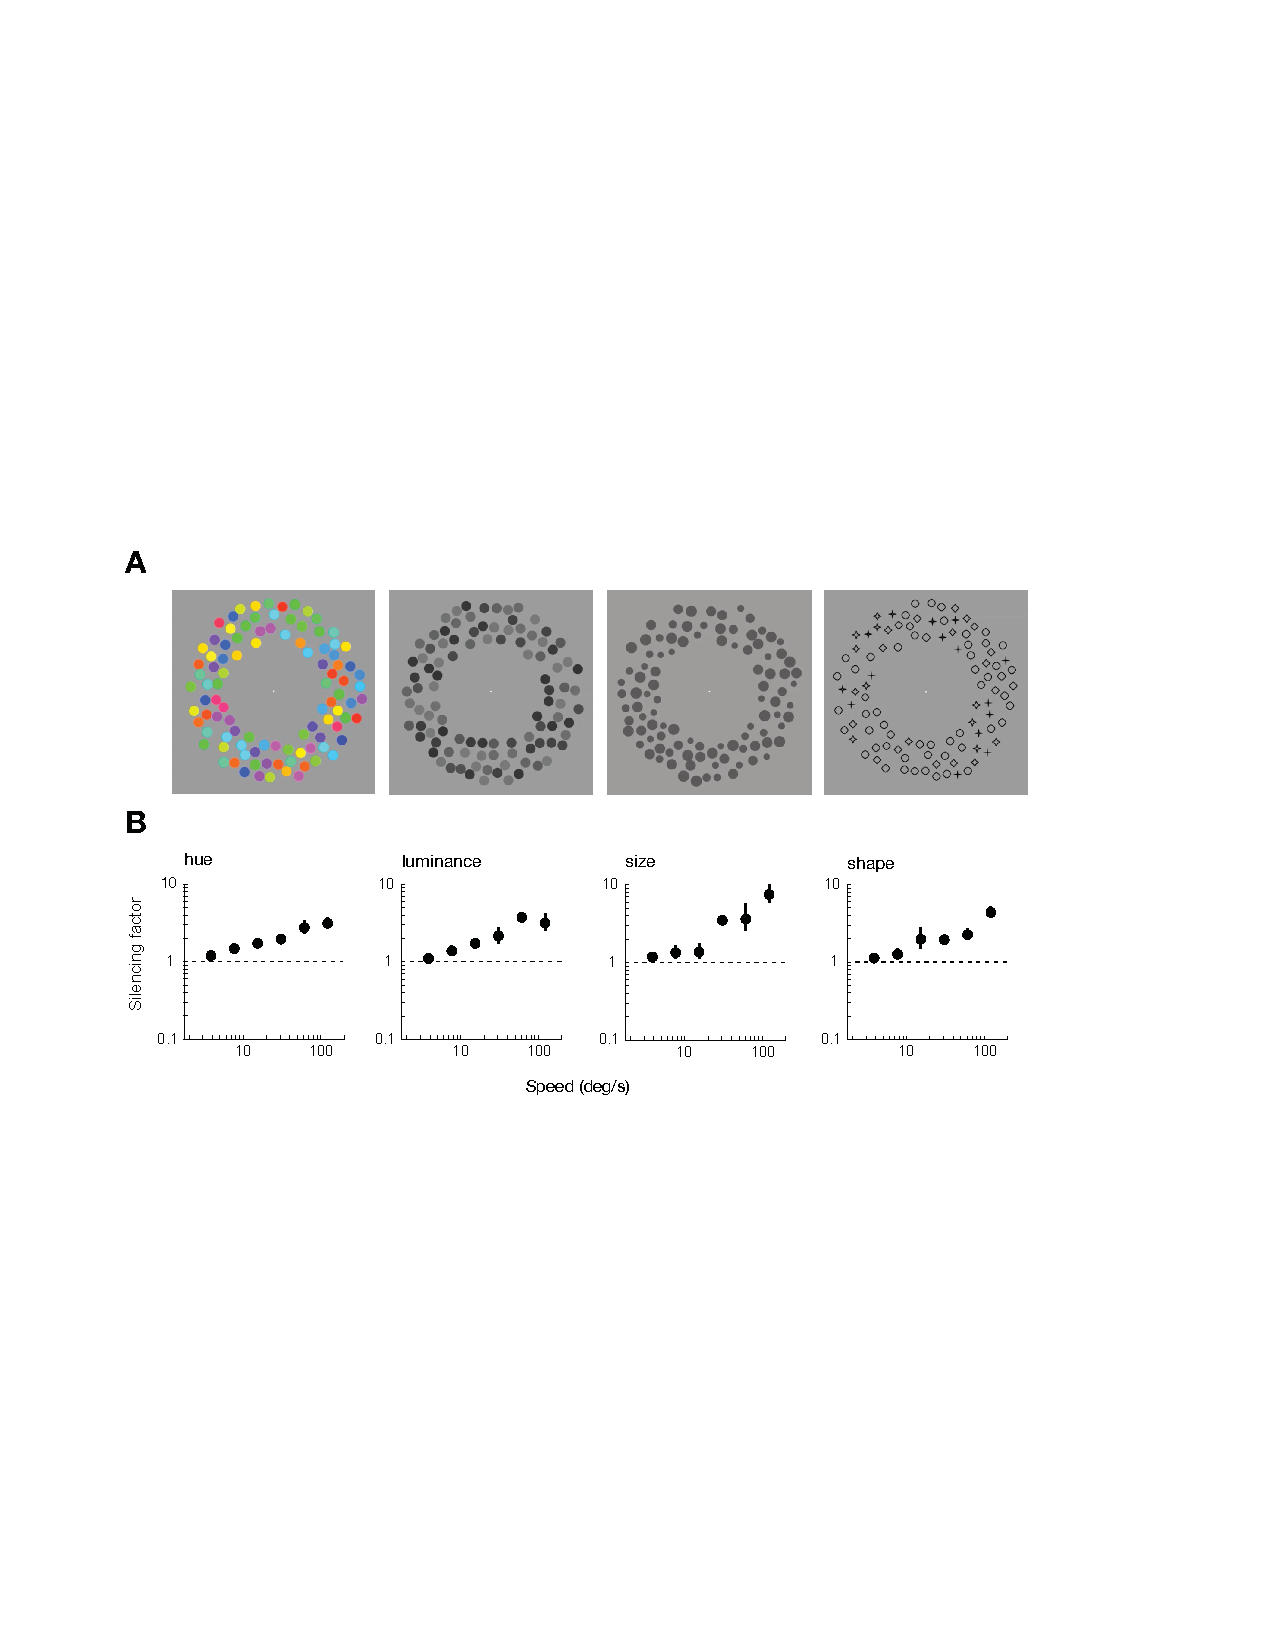
\includegraphics[width=\textwidth]{figures/fig1}
\caption[Short figure name.]{This is a figure that floats inline and here is its caption.
\label{fig:myInlineFigure}}
\end{figure}



%% Requires fltpage2 package
%%
% \begin{FPfigure}
% 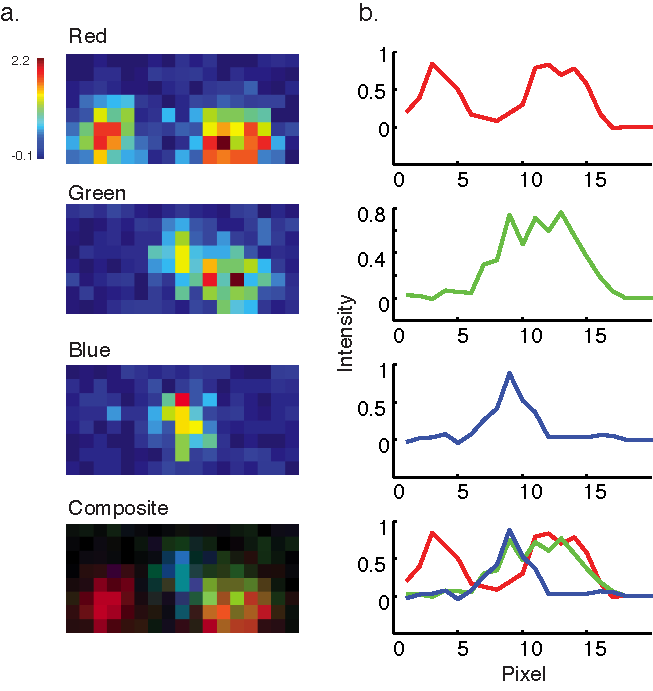
\includegraphics[width=\textwidth]{figures/fullpage}
% \caption[Short figure name.]{This is a full page figure using the FPfigure command. It takes up the whole page and the caption appears on the preceding page. Its useful for large figures. Harvard's rules about full page figures are tricky, but you don't have to worry about it because we took care of it for you. For example, the full figure is supposed to have a title in the same style as the caption but without the actual caption. The caption is supposed to appear alone on the preceding page with no other text. You do't have to worry about any of that. We have modified the fltpage package to make it work. This is a lengthy caption and it clearly would not fit on the same page as the figure. Note that you should only use the FPfigure command in instances where the figure really is too large. If the figure is small enough to fit by the caption than it does not produce the desired effect. Good luck with your thesis. I have to keep writing this to make the caption really long. LaTex is a lot of fun. You will enjoy working with it. Good luck on your post doctoral life! I am looking forward to mine. \label{fig:myFullPageFigure}}
% \end{FPfigure}
% \afterpage{\clearpage}
